% !TeX encoding = UTF-8
% !TeX program = pdflatex

\documentclass[11pt]{article}
\usepackage{graphicx}

\title{{\bf My crypto libraries} \\ \bigskip \large HW4 - CNS Sapienza}
\date{2019-11-28}
\author{Valerio Coretti 1635747}
\pagenumbering{roman}

\begin{document}
\maketitle

\section{Introduction}
In this paper, we address the issue of cryptographic libraries. Today cryptography plays a key role in cybersecurity. For this reason, there are many cryptographic libraries for different programming languages available to developers.

In the following sections we will present an experiment made with four different cryptographic libraries: {\em OpenSSL, WolfSSL, PyCryptodome, Cryptography}. The first two are used with {\em C} programming language and the other two with {\em Python}.

First, we will do a brief presentation of the four libraries and then we will do a comparison of the main mechanism and the performances.

The comparison has been conducted with a MacBook Pro, Intel Core i7 processor, and 8GB of RAM. The speed is measured in seconds.

\section{Crypto libraries}
In this section, we will present the libraries used and how to install them.

\subsection{OpenSSL}
OpenSSL is the most popular cryptographic library. It is an open-source project written in C programming language and contains an implementation of the SSL and TLS protocols. Used by the applications that secure communications over computer networks and also widely used by Internet servers.

OpenSSL supports a number of different cryptographic algorithms:
\begin{itemize}
 \item {\em Ciphers}: AES, Blowfish, Camellia, Chacha20, Poly1305, SEED, DES, IDEA, RC2, RC4, RC5, Triple DES, SM4 [4]
 \item {\em Cryptographic hash functions}: MD5, MD4, MD2, SHA1, SHA2, SHA3, RIPEMD-160, MDC2, BLAKE2, Whirlpool, SM3 [4]
 \item {\em Public-key cryptography}: RSA, DSA, Diffie Hellman key exchange, Elliptic curve, X25519, Ed25519, X448, Ed448, SM2 [4]
\end{itemize}

We use OpenSSL $1.1.1d$. For Mac OSx the installation involves several steps:
\begin{itemize}
\item Installation:
\begin{figure}[!ht]
 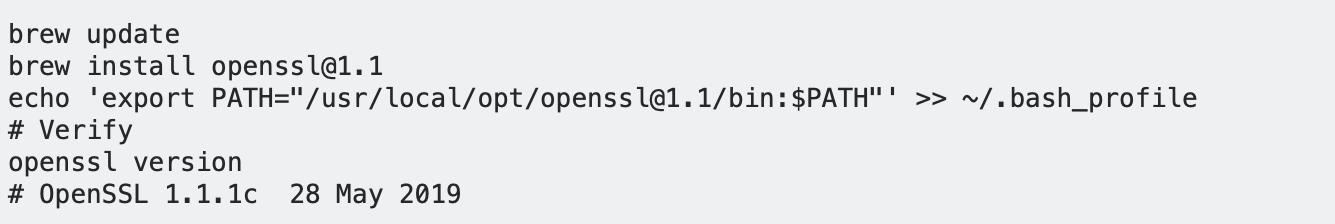
\includegraphics[width=1\textwidth]{pic1-hw4-1635747}
 \label{fig:OpenSSL Mac Installation}
\end{figure}

\item Compilation:\newline
{\em gcc$\;\;$-L/usr/local/opt/openssl/lib$\;\;$-I/usr/local/opt/openssl/include$\;\;$file.c -o file -lssl -lcrypto}
\item Implementation: the best ways to implement OpenSSL is to use the the high-level interface EVP. This provide a large range of function that can be used for our purpose.

\end{itemize}

To use OpenSSL is a good idea to see the official documentation but for very strong developers it is useful to see also the source code available in the GitHub repository:\newline
\verb|https://github.com/openssl/openssl|\newline
\verb|https://www.openssl.org/docs/man1.1.1/man3/|

\subsection{WolfSSL}
WolfSSL is a small, portable, embedded SSL/TLS library targeted for use by embedded systems developers. It is an Open Source implementation of TLS, written in ANSI C. A predecessor of wolfSSL is yaSSL, a C++ based SSL library for {\em embedded environments} and real-time operating systems with constrained resources. [2]

WolfSSL, formerly CyaSSL, is about 10 times smaller than yaSSL and up to 20 times smaller than OpenSSL. By default, wolfSSL uses the cryptographic services provided by {\em WolfCrypt}. This Provides RSA, ECC, DSS, Diffie Hellman, EDH, NTRU, DES, Triple DES, AES (CBC, CTR, CCM, GCM), Camellia, IDEA, ARC4, ChaCha20, MD2, MD4, MD5, SHA1, SHA2, SHA3, BLAKE2, RIPEMD160, Poly1305, Random Number Generation, Large Integer support, and base64 encoding, decoding.[1]

For our purpose, we use wolfCrypt services. Let's start to see some useful commands. Note that the following commands are used in Mac OSx for other operating systems it is advisable to look at the official documentation.
\begin{itemize}
\item Installation: {\em brew install wolfssl}
\item Compilation: {\em gcc file.c -o file -lm -lwolfssl}
\item Implementation: All we need for the implementation is in the GitHub repository (see later) and in the documentation. But it good to know that unlike OpenSSL, in WolfSSL the input file must be padded otherwise we have an error in the execution.
\end{itemize}

WolfSSL and wolfCrypt are available also for Python and Java. As first time we searched examples of use and source code in the GitHub repository and the official documentation:\newline
- \verb|https://github.com/wolfSSL|\newline
- \verb|https://www.wolfssl.com/doxygen/group__AES.html|

\subsection{PyCryptodome}
PyCryptodome is a Python package that provides a low-level cryptographic primitives. It is a fork of the native package PyCrypto. It supports Python 2.6 and 2.7, Python 3.4 and newer, and PyPy. It brings the following cryptographic features:

\begin{itemize}
 \item {\em Ciphers}: AES, Blowfish, Camellia, Chacha20, Poly1305, SEED, DES, IDEA, RC2, RC4, RC5, Triple DES, SM4, Salsa20 [6]
 \item {\em Modes of operations}: ECB, CBC, CFB, OFB, CTR, CCM (AES only), EAX, GCM (AES only), SIV (AES only), OCB (AES only), ChaCha20, Poly1305 [6]
 \item {\em Cryptographic hash functions}: MD5, SHA1, SHA2, SHA3, RIPEMD 160, BLAKE2, Keccak [6]
 \item {\em Public-key cryptography}: RSA, DSA, ECC, ElGamal (legacy) [6]
 \item {\em Key derivation}: PBKDF2, scrypt, HKDF
\end{itemize}

Now analyze the main steps to implement this cryptographic library:
\begin{itemize}
\item Installation: {\em pip3 install pycryptodome}
\item Compilation: {\em python3 file.py}
\item Implementation: as we expected python implementation is simpler than C, but you still need to pay attention to some details. First of all, like WolfCrypt pycrypto needs the manual padding, furthermore when we want to encrypt/decrypt a file we must convert this in base64 encoding so that it can take everything as binary. (see at source code)
\end{itemize}

\subsection{Cryptography}
Cryptography is a package that provides cryptographic recipes and primitives to Python developers. It supports Python 2.7, Python 3.4+, and PyPy 5.4+.

Cryptography is divided into two levels. The first is high-level that don't require configuration choices. These are safe and easy to use and don’t require developers to make many decisions. The other provides low-level cryptographic primitives. They require some knowledge of the cryptographic concepts. Because of the potential danger in working at this level, this is referred to as the {\em hazardous materials} or {\em hazmat} layer. [7]

This library implements the main features of modern cryptography. A very good list of these features it can be reachable directly in the API documentation:\newline
\verb|https://cryptography.io/en/latest/hazmat/primitives/|

Now analyze the main steps to implement this cryptographic library:
\begin{itemize}
\item Installation: {\em pip3 install cryptography}
\item Compilation: {\em python3 file.py}
\item Implementation: the considerations about the implementation is similar to pycryptodome.
\end{itemize}

\section{Experimentation}
We create two scripts, the first in C programming language called

{\em my\_crypto\_library$-$hw4$-$1635747.c}, to test OpenSSL and WolfSSL, and the other in Python {\em my\_crypto\_library$-$hw4$-$1635747.py}, to test PyCryptodome and Cryptography. We did several experiments with these libraries. Scripts take in input a file that can be of whatever size and type (images, binary, text, ...). We used AES with CBC mode for all tests and we choose a pseudo-random key of 256 bit and a random iv of 128 bit.

\subsection{Speed time}
First of all we test de encryption and decryption speed with three different file size: {\em 100KB, 5MB, 140MB}.

\begin{figure}[!ht]
 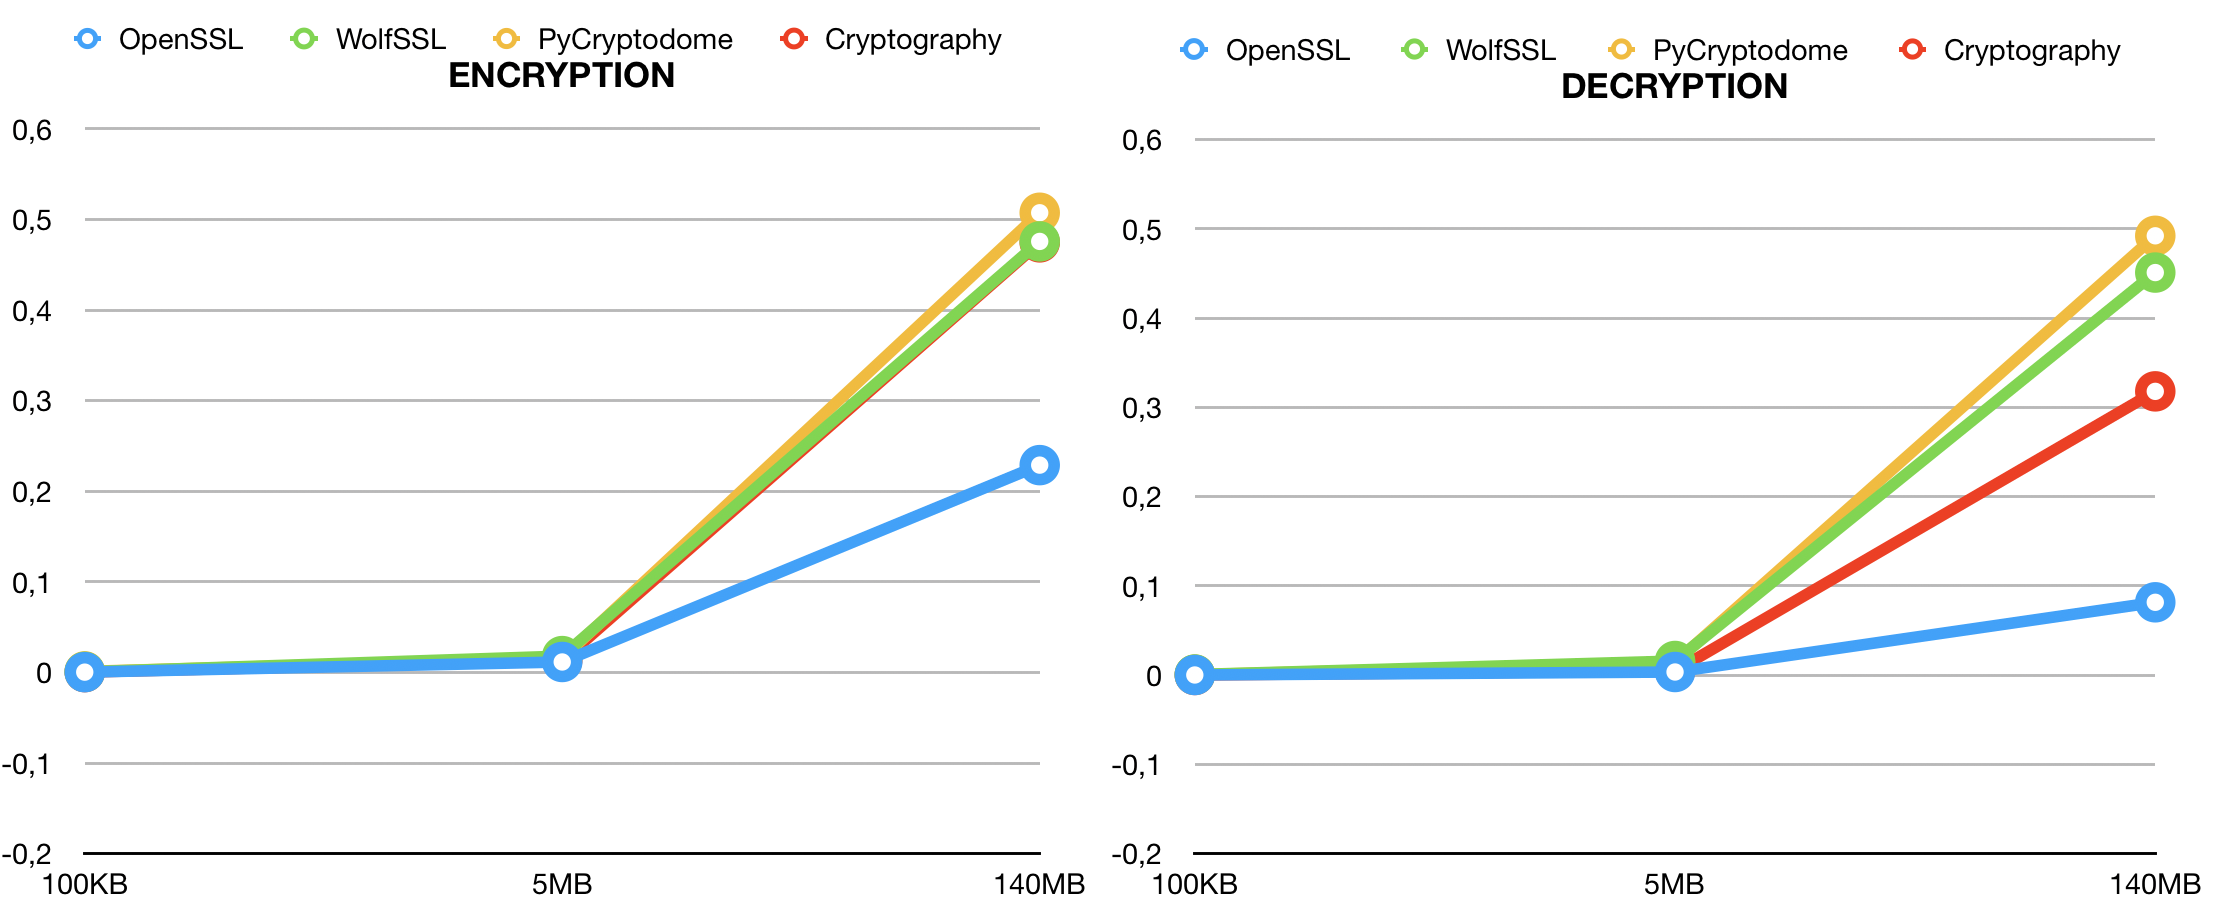
\includegraphics[width=1\textwidth]{pic2-hw4-1635747}
 \label{fig:Encryption and Decryption speed}
\end{figure}

As we can see OpenSSL is the fastest for both encrypt and decrypt, for the other libraries we have WolfSSL and PyCryptodome that has very similar speed time and an interesting thing is that the encryption and decryption have about the same timing, this means probably that they don't implement the parallelization of the decryption. Cryptography compared to these last two presents improvements in the decryption. For completeness in the next figure, we report the speed ratio that is the relation between encryption and decryption time. However, these differences are found as the size of the files increases, as we can see for small files all libraries behave more or less in the same way.

\begin{figure}[!ht]
 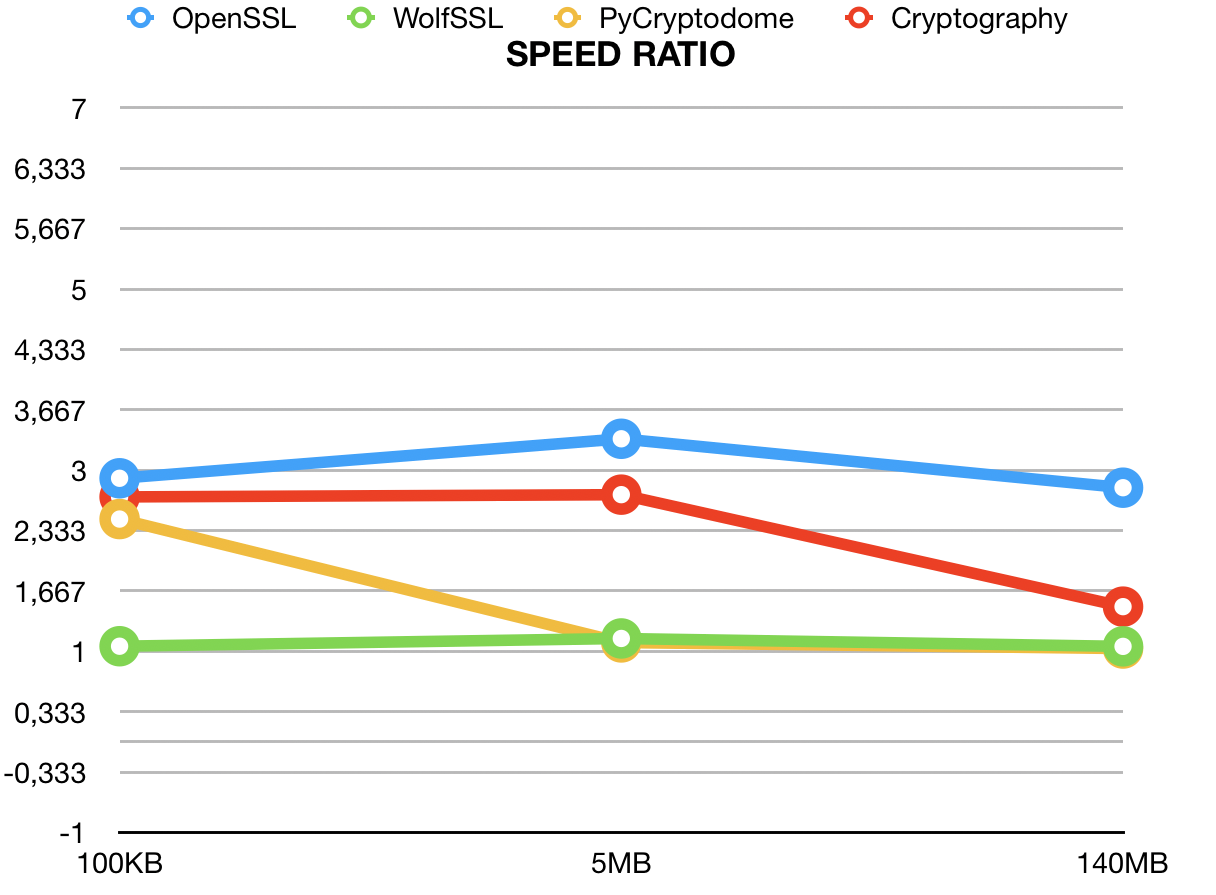
\includegraphics[width=1\textwidth]{pic3-hw4-1635747}
 \label{fig:Speed ratio}
\end{figure}

\subsection{Combinations}
In this paragraph, we will see a particular experiment where we tried to encrypt with one library and decrypt with another. Unfortunately, most of the experiments have failed. In the following image, we show the compatibility between the various libraries.

\begin{figure}[!ht]
 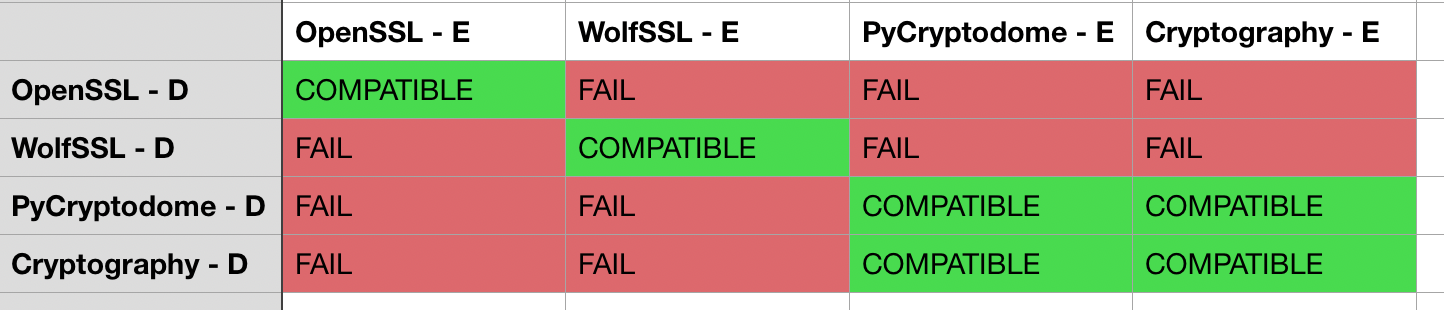
\includegraphics[width=1\textwidth]{pic4-hw4-1635747}
 \label{fig:Compatibility}
\end{figure}

As we can see the combinations with OpenSSL and WolfSSL fail in every case while the operations of the analyzed Python libraries can be combined.

\section{Conclusion}
In this paper, we have seen a presentation of four cryptographic libraries in terms of technical details, performances and finally a combination of these. OpenSSL is surely the best of the four and it is the one that presents the biggest range of functionality. It can be used for any purpose in cryptography. It also has the best performances in terms of encryption/decryption speed.

WolfSSL has bad performances about speed but its power is the smaller size, indeed it is about twenty times smaller than OpenSSL. For this reason, it is thought for embedded systems.

Indeed if we want to use cryptographic libraries in Python, surely Cryptography is the best choice. It has better performances then WolfSSL and worse than OpenSSL.

Finally, we have seen PyCryptodome. It has similar performances of WolfSSL but in general, using Python, Cryptography is for sure the best.


\vfill
\begin{thebibliography}{99}

\bibitem{wiki1}
{\em Comparison of cryptography libraries - Wikipedia}. \newline
 \verb|https://en.wikipedia.org/wiki/Comparison_of_cryptography_libraries|

\bibitem{wiki2}
{\em WolfSSL - Wikipedia}. \newline
 \verb|https://en.wikipedia.org/wiki/WolfSSL|

\bibitem{doc1}
{\em WolfSSL - Documentation}. \newline
 \verb|https://www.wolfssl.com/docs/|

\bibitem{wiki4}
{\em OpenSSL - Wikipedia}. \newline
 \verb|https://en.wikipedia.org/wiki/OpenSSL|

\bibitem{doc2}
{\em OpenSSL Documentation}. \newline
\verb|https://www.openssl.org/docs/manmaster/man3/|

\bibitem{doc3}
{\em Pycryptodome Documentation}. \newline
\verb|https://www.pycryptodome.org/en/latest/|

\bibitem{doc3}
{\em Cryptography Documentation}. \newline
\verb|https://cryptography.io/en/latest/|

\end{thebibliography}
\end{document}

